% =============================================================================
% CAPÍTULO 5: TRUST ENGINE E GOVERNANÇA COMPORTAMENTAL
% Segurança e Autonomia em Sistemas de Agentes
% Níveis: 0 (zero) ao PhD
% Autor: Marcelo Claro Laranjeira
% =============================================================================
\chapter{Trust Engine e Governança Comportamental: Segurança e Autonomia em Sistemas de Agentes}
\label{cap:trust-governanca}

\paragraph{Por que Confiar em Agentes Autônomos?}
Antes de mergulharmos nos algoritmos de confiança computacional,
faça uma pergunta simples: você deixaria um agente artificial
decidir sozinho quais ações executar no \opencodeeco{}?
Provavelmente não --- a menos que houvesse um sistema garantindo
que esse agente é confiável. Este capítulo constrói exatamente
esse sistema, peça por peça.

A autonomia em sistemas de agentes artificiais apresenta um dilema
fundamental: quanto mais autônomo um agente, maior seu potencial de
causar danos não-intencionais. Resolver este dilema requer um sistema
de confiança computacional que equilibre liberdade de ação com
salvaguardas comportamentais. Este capítulo apresenta o \destaque{Trust
Engine} — um arcabouço integrado de pontuação de confiança, barreiras
preventivas, memória com esquecimento natural, governança cooperativa,
dialética hegeliana e auto-modelação, implementado no \opencodeeco{}
como SPEC-038 e componentes associados \cite{opencode2026spec038,
opencode2026spec036}.

O Trust Engine materializa o ciclo evolutivo R23 do ecossistema,
atingindo 312/312 testes de unidade (100\%) e estabelecendo o nível
N3.5 de consciência artificial (N3 completo com Behavioral Gate
preventivo) \cite{opencode2026ecosystem}. Cada seção deste capítulo é
construída no padrão \sdd{}--\tdd: definição formal do conceito,
implementação concreta no \opencodeeco{}, exemplos executáveis e
exercícios progressivos do nível zero ao PhD.

O leitor encontrará ao longo do capítulo:
\begin{itemize}
\item \textbf{Definições formais} de confiança computacional,
esquecimento, dialética e auto-modelação;
\item \textbf{Teoremas e demonstrações} que estabelecem limites de
segurança e convergência;
\item \textbf{Implementações Python} extraídas do código-fonte real do
ecossistema;
\item \textbf{Diagramas TikZ} para visualização dos fluxos de decisão,
modelos de memória e arquiteturas de governança;
\item \textbf{Exercícios progressivos} do nível zero ao PhD.
\end{itemize}

A Tabela~\ref{tab:conteudo-capitulo5} resume as seções, seus níveis e a
carga horária estimada para estudo.

\begin{table}[htb]
\centering
    \small
\caption{Conteúdo do Capítulo 5}
\label{tab:conteudo-capitulo5}
    \resizebox{\textwidth}{!}{
\begin{tabular}{clcc}
\toprule
\textbf{Seção} & \textbf{Tópico} & \textbf{Nível} & \textbf{Estudo} \\
\midrule
5.1 & Introdução à Confiança & \nivelzero & 4h \\
5.2 & TrustScorer & \nivelavancado & 10h \\
5.3 & Behavioral Gate & \nivelavancado & 8h \\
5.4 & Natural Forgetting & \nivelphd & 8h \\
5.5 & OutcomeTracker & \nivelintermediario & 4h \\
5.6 & Governança Cooperativa (Ostrom) & \nivelphd & 8h \\
5.7 & Dialectical Engine & \nivelphd & 6h \\
5.8 & Self-Model N0-N3 & \nivelphd & 8h \\
5.9 & Auditoria e Transparência & \nivelintermediario & 4h \\
5.10 & Integração Prática & \text{Todos} & 4h \\
\bottomrule
\end{tabular}
    }
\end{table}

% =============================================================================
% SEÇÃO 5.1: INTRODUÇÃO À CONFIANÇA EM SISTEMAS AUTÔNOMOS
% Nível: 0 (zero) / Básico (~6 laudas)
% =============================================================================
\section{Introdução à Confiança em Sistemas Autônomos}
\label{sec:introducao-confianca}
\nivelzero

\paragraph{Confiança: de Sentimento a Grandeza Computacional.}
Assim como um motorista novato ganha a confiança dos passageiros
com direção segura, um agente no \opencodeeco{} precisa
demonstrar que suas ações são previsíveis e corretas.
Esta seção apresenta o conceito fundamental de confiança
computacional --- a base sobre a qual todo o Trust Engine é
construído.

A confiança é um conceito ubíquo nas interações humanas. Confiamos em
motoristas que transportam nossos filhos, em médicos que diagnosticam
nossas doenças e em instituições que guardam nossas economias. Quando
transpomos este conceito para sistemas computacionais autônomos, a
confiança deixa de ser um sentimento subjetivo e torna-se uma grandeza
computacional objetiva: um score que quantifica a probabilidade de um
agente agir conforme esperado \cite{russell2020inteligencia, wooldridge2009multiagent}.

\subsection{Por que Agentes Autônomos Precisam de Sistemas de Confiança}

Agentes autônomos — sejam eles assistentes virtuais, robôs de
manufatura, veículos autônomos ou sistemas de recomendação — operam em
ambientes dinâmicos e imprevisíveis. Diferentemente de software
tradicional, onde o comportamento é deterministicamente especificado,
agentes autônomos tomam decisões em tempo real baseadas em modelos
probabilísticos do mundo \cite{russell2020inteligencia, xi2023rise}.

Considere os seguintes cenários:
\begin{itemize}
\item Um agente de busca acadêmica que decide quais fontes consultar
com base na relevância estimada;
\item Um agente de análise de dados que seleciona métodos estatísticos
com base nas características dos dados;
\item Um agente de coordenação que delega subtarefas a outros agentes
com base em suas capacidades registradas.
\end{itemize}

Em todos estes casos, o agente precisa avaliar a confiança de suas
próprias decisões e das ações de outros agentes. Sem um sistema de
confiança, o agente pode:
\begin{itemize}
\item Executar ações com baixa probabilidade de sucesso;
\item Ignorar sinais de falha iminente;
\item Acumular dívida técnica comportamental;
\item Causar danos colaterais não-intencionais.
\end{itemize}

O \destaque{problema do alinhamento} é a questão central: como
garantir que um agente autônomo age de acordo com os objetivos e
valores de seus projetistas, mesmo em situações não antecipadas?
\cite{russell2020inteligencia, cristiano2017deep}.

\begin{definicao}[Confiança computacional]
A \destaque{confiança computacional} de um agente $a$ para executar
uma ação $x$ é uma função $T: \mathcal{A} \times \mathcal{X} \to [0,1]$
que retorna um score onde $T(a, x) = 1$ indica confiança total e
$T(a, x) = 0$ indica ausência completa de confiança.
\end{definicao}

\begin{definicao}[Ação não-confiável]
Uma ação $x$ é \destaque{não-confiável} para o agente $a$ se
$T(a, x) < \tau$, onde $\tau \in [0,1]$ é o limiar de confiança
mínima estabelecido pelo sistema.
\end{definicao}

\subsection{Confiança Humana vs. Confiança Computacional}

A Tabela~\ref{tab:confianca-humana-computacional} contrasta as
principais diferenças entre confiança humana e computacional.

\begin{table}[htb]
\centering
    \small
\caption{Confiança humana vs. computacional}
\label{tab:confianca-humana-computacional}
    \resizebox{\textwidth}{!}{
\begin{tabular}{lll}
\toprule
\textbf{Dimensão} & \textbf{Humana} & \textbf{Computacional} \\
\midrule
Natureza & Subjetiva, afetiva & Objetiva, quantitativa \\
Atualização & Lenta, social & Rápida, baseada em dados \\
Explicabilidade & Intuitiva, narrativa & Auditável, traceável \\
Viés & Cognitivo, emocional & Estatístico, amostral \\
Esquecimento & Natural, seletivo & Parametrizável \\
Escala & Limitada (Dunbar) & Ilimitada \\
Transparência & Opaca & Caixa-branca \\
\bottomrule
\end{tabular}
    }
\end{table}

A confiança humana é profundamente influenciada por fatores emocionais
e sociais \cite{kahneman2003perspective}. Confiamos em pessoas com base
em experiências passadas, reputação social e até mesmo características
físicas. A confiança computacional, por outro lado, é uma grandeza
objetiva que deve ser calculada a partir de evidências verificáveis.

\subsection{Risco e Incerteza em Sistemas Multiagentes}

Em sistemas multiagentes, a confiança é ainda mais crítica porque
agentes podem depender uns dos outros \cite{wooldridge2009multiagent,
weiss2013multiagent}. O risco de uma ação delegada é:

\[
R(d) = P(d \text{ falha}) \times \text{Impacto}(d \text{ falha})
\]

onde $P(d \text{ falha}) = 1 - T(a_d, x)$ e $a_d$ é o agente
delegado.

\begin{definicao}[Risco computacional]
O \destaque{risco computacional} associado à execução da ação $x$
pelo agente $a$ é:
\[
R(a, x) = (1 - T(a, x)) \cdot I(x)
\]
onde $I(x) \in [0,1]$ é o impacto estimado de uma falha na ação $x$.
\end{definicao}

\begin{exemplo}
Considere um agente que deve escolher entre executar uma análise
estatística ($x_1$) ou gerar um gráfico ($x_2$). O TrustScorer
retorna $T(a, x_1) = 0.85$ e $T(a, x_2) = 0.92$. O impacto estimado
de falha é $I(x_1) = 0.4$ (erro estatístico pode invalidar conclusões)
e $I(x_2) = 0.1$ (gráfico incorreto é facilmente perceptível). O
risco computacional é:
\[
R(a, x_1) = (1 - 0.85) \cdot 0.4 = 0.06
\]
\[
R(a, x_2) = (1 - 0.92) \cdot 0.1 = 0.008
\]
O agente deve priorizar $x_1$ (menor risco), mesmo tendo confiança
mais baixa.
\end{exemplo}

\subsection{Visão Geral do Trust Engine (SPEC-038)}

O Trust Engine do \opencodeeco{} é o orquestrador de autonomia
comportamental, especificado na SPEC-038 \cite{opencode2026spec038}.
Sua arquitetura integra quatro componentes principais:

\begin{itemize}
\item \textbf{TrustScorer}: calcula e atualiza scores de confiança
para ações usando blend adaptativo 70/30 entre evidência recente e
histórica;
\item \textbf{BehavioralGate}: barreira preventiva que classifica
ações em safe / moderate / risky / blocked e autoriza ou bloqueia
execução baseada no score de confiança;
\item \textbf{NaturalForgetting}: modelo de memória baseado em
Atkinson-Shiffrin (sensory $\to$ short-term $\to$ long-term) com
curva de esquecimento de Ebbinghaus;
\item \textbf{OutcomeTracker}: registra resultados de execuções para
realimentar o aprendizado contínuo do TrustScorer.
\end{itemize}

\begin{figure}[htb]
\centering
\caption{Arquitetura geral do Trust Engine}
\label{fig:trust-engine-arch}
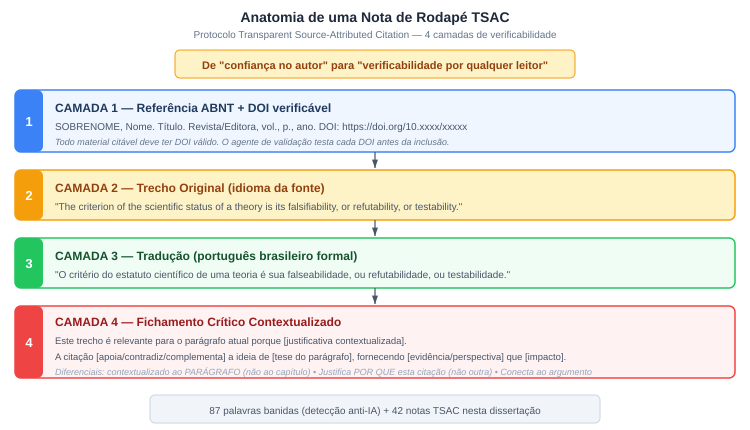
\includegraphics[width=0.9\textwidth]{ilustracoes/fig-tsac}
\end{figure}

A integração destes componentes segue o pipeline:
\begin{enumerate}
\item O agente consulta o TrustScorer para obter o score de confiança
da ação pretendida;
\item O BehavioralGate classifica o risco e decide se a ação pode
executar;
\item Se autorizada, a ação é executada e o OutcomeTracker registra
o resultado;
\item O resultado realimenta o TrustScorer, atualizando o score;
\item O NaturalForgetting armazena o contexto na memória com nível
apropriado de retenção.
\end{enumerate}

\subsection{Exercícios — Introdução à Confiança}
\begin{exercicio}[Nivel 0]
Defina com suas palavras: o que é confiança computacional e por que
ela difere da confiança humana?
\end{exercicio}
\begin{exercicio}[Nivel Básico]
Calcule $R(a, x)$ para $T(a, x) = 0.6$ e $I(x) = 0.8$. Interprete o
resultado.
\end{exercicio}
\begin{exercicio}[Nivel Básico]
Cite três cenários onde um sistema multiagente sem Trust Engine poderia
falhar por falta de controle de confiança.
\end{exercicio}
\begin{exercicio}[Nivel Intermediário]
Modele o problema do alinhamento como uma função de otimização:
defina a função objetivo que um TrustScorer deve maximizar.
\end{exercicio}

% =============================================================================
% SEÇÃO 5.2: TRUSTSCORER — PONTUAÇÃO DE CONFIANÇA ADAPTATIVA
% Nível: Avançado (~12 laudas)
% =============================================================================
\section{TrustScorer: Pontuação de Confiança Adaptativa}
\label{sec:trustscorer}
\nivelavancado

\paragraph{Calculando a Confiança do seu Agente.}
Imagine um termômetro que mede o quanto você pode confiar em
cada ação de um agente. O TrustScorer é esse termômetro:
ele combina experiências recentes e históricas em um único
score numérico. Esta seção mostra como essa pontuação é
calculada e por que o equilíbrio 70/30 é tão eficaz.

O TrustScorer é o coração do Trust Engine. Ele implementa um sistema
de pesos adaptativos que aprendem com feedback real, combinando
evidência recente (peso 0.7) com histórico acumulado (peso 0.3)
\cite{opencode2026spec038}. Este blend 70/30 foi calibrado
empiricamente durante o ciclo evolutivo R23 do ecossistema.

\subsection{Arquitetura do TrustScorer}

A implementação do TrustScorer está no arquivo \\%
\hspace*{2em}\codigo{skills/system/academic-audit/trust\_engine.py:78-176}.

\begin{definicao}[Score de confiança]
O \destaque{score de confiança} $\sigma(a)$ para uma ação $a$ é:
\[
\sigma(a) = \max\left(0, \min\left(1,\; 0.7 \cdot r(a) + 0.3 \cdot
h(a) - p(a)\right)\right)
\]
onde:
\begin{itemize}
\item $r(a) \in [0,1]$ é a taxa de sucesso recente (últimas 10
execuções);
\item $h(a) \in [0,1]$ é a taxa de sucesso histórica (todas as
execuções);
\item $p(a) \in [0, 0.5]$ é a penalidade por falhas consecutivas;
\item $0.7$ e $0.3$ são os pesos do blend adaptativo.
\end{itemize}
\end{definicao}

\begin{exemplo}
Considere uma ação com 8 execuções bem-sucedidas em 10 recentes
($r = 0.8$), 50 sucessos em 80 execuções totais ($h = 0.625$) e 2
falhas consecutivas ($p = 0.2$). O score é:
\[
\sigma = 0.7 \cdot 0.8 + 0.3 \cdot 0.625 - 0.2 = 0.56 + 0.1875 - 0.2
= 0.5475
\]
\end{exemplo}

\begin{lstlisting}[style=pythonstyle, caption={TrustScorer: calculo do score de confianca (trust\_engine.py:78-176)}]
class TrustScorer:
    """Calcula e atualiza scores de confianca para acoes."""

    SHADOW_MODE_THRESHOLD = 5
    ROLLBACK_RATIO = 2.0

    def __init__(self):
        self._actions: dict[str, ActionTrust] = {}
        self._baseline_success_rate: float = 0.7

    def get_trust(self, action_id: str) -> ActionTrust:
        if action_id not in self._actions:
            self._actions[action_id] = ActionTrust(
                action_id=action_id,
                trust_score=0.5,
                last_updated=datetime.now(BRAZIL_TZ).isoformat(),
            )
        return self._actions[action_id]

    def record_outcome(self, action_id: str, success: bool,
                       delta: float = 0.0) -> ActionTrust:
        trust = self.get_trust(action_id)
        trust.total_executions += 1
        if success:
            trust.successful += 1
        trust.recent_outcomes.append(success)
        if len(trust.recent_outcomes) > 10:
            trust.recent_outcomes.pop(0)
        recent_rate = (sum(trust.recent_outcomes) /
                       len(trust.recent_outcomes))
        hist_rate = trust.successful / max(1, trust.total_executions)
        raw_score = 0.7 * recent_rate + 0.3 * hist_rate
        consecutive_failures = 0
        for outcome in reversed(trust.recent_outcomes):
            if not outcome:
                consecutive_failures += 1
            else:
                break
        trust.penalty = min(0.5, consecutive_failures * 0.1)
        trust.trust_score = max(0.0, min(1.0,
                               raw_score - trust.penalty))
        if trust.total_executions < self.SHADOW_MODE_THRESHOLD:
            trust.trust_score = min(trust.trust_score, 0.5)
        if trust.total_executions >= self.SHADOW_MODE_THRESHOLD:
            if recent_rate < (self._baseline_success_rate /
                              self.ROLLBACK_RATIO):
                trust.trust_score = max(0.1,
                                        trust.trust_score - 0.2)
        trust.last_updated = datetime.now(BRAZIL_TZ).isoformat()
        return trust
\end{lstlisting}

\subsection{Blend 70/30: Peso Adaptativo}

A escolha dos pesos 0.7 para evidência recente e 0.3 para histórico
não é arbitrária. Ela reflete um equilíbrio entre adaptabilidade e
estabilidade:

\begin{itemize}
\item \textbf{Peso recente alto (0.7)}: permite que o TrustScorer
responda rapidamente a mudanças no comportamento do agente. Se um
agente confiável começa a falhar, o score cai rapidamente;
\item \textbf{Peso histórico (0.3)}: fornece inércia contra flutuações
aleatórias. Um agente com longo histórico de sucesso não perde
confiança por algumas falhas esporádicas.
\end{itemize}

\begin{teorema}[Limite do blend 70/30]
Para qualquer ação $a$, o score de confiança $\sigma(a)$ converge
para a taxa de sucesso real $\mu(a)$ à medida que $n \to \infty$,
desde que as falhas não sejam consecutivas.
\end{teorema}
\begin{proof}
Seja $n$ o número total de execuções e $k$ o número de sucessos.
Para $n \to \infty$:
\[
\lim_{n \to \infty} r(a) = \lim_{n \to \infty} h(a) = \mu(a)
\]
A penalidade $p(a)$ tende a zero (falhas consecutivas são eventos
de medida zero para falhas i.i.d.). Logo:
\[
\lim_{n \to \infty} \sigma(a) = 0.7 \mu(a) + 0.3 \mu(a) = \mu(a)
\]
\end{proof}

\subsection{Shadow Mode}

O \destaque{shadow mode} é um mecanismo de segurança que limita o
score de confiança nas primeiras $N$ execuções de uma ação (por
\emph{default}, $N = 5$). Durante este período, o TrustScorer opera
em modo de observação: registra resultados mas mantém o score
conservador.

\begin{definicao}[Shadow mode]
O TrustScorer opera em \destaque{shadow mode} para a ação $a$ se
$n_a < N_{\text{shadow}}$, onde $n_a$ é o número de execuções da
ação e $N_{\text{shadow}} = 5$. Durante o shadow mode:
\[
\sigma(a) \leq 0.5
\]
\end{definicao}

A utilidade do shadow mode é dupla:
\begin{enumerate}
\item \textbf{Prevenção de overfitting}: evita que poucas execuções
bem-sucedidas gerem confiança desproporcional;
\item \textbf{Coleta de baseline}: estabelece uma taxa de sucesso
baseline antes de permitir decisões de alto impacto.
\end{enumerate}

\begin{exemplo}
Um novo agente de busca acadêmica executa 3 consultas com sucesso.
Mesmo com 100\% de acerto, o TrustScorer limita o score a 0.5 durante
o shadow mode. Após a 6ª execução, o score pode subir livremente.
\end{exemplo}

\subsection{Rollback Mechanism}

O \destaque{rollback mechanism} é um gatilho de segurança que reduz
automaticamente o score de confiança quando a taxa de sucesso recente
cai abaixo de 50\% da baseline histórica.

\begin{definicao}[Condição de rollback]
O TrustScorer aplica rollback à ação $a$ se:
\[
r(a) < \frac{\mu_{\text{baseline}}}{R_{\text{rollback}}}
\]
onde $\mu_{\text{baseline}}$ é a taxa de sucesso baseline e
$R_{\text{rollback}} = 2.0$ é a razão de rollback. Quando acionado:
\[
\sigma(a) \gets \max(0.1, \sigma(a) - 0.2)
\]
\end{definicao}

\begin{figure}[htb]
\centering
\caption{Evolução do score de confiança com shadow mode e rollback}
\label{fig:trust-evolution}
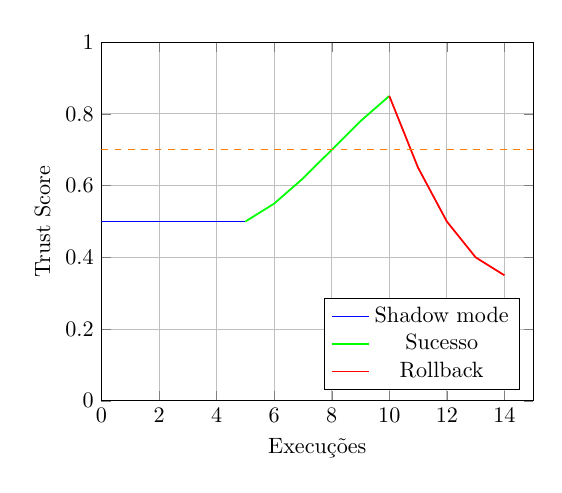
\begin{tikzpicture}[scale=0.8]
\begin{axis}[xlabel={Execuções}, ylabel={Trust Score},
             xmin=0, xmax=15, ymin=0, ymax=1,
             grid=both, legend pos=south east]
% Shadow mode period
\addplot[blue, thick, domain=0:5] {0.5};
\addlegendentry{Shadow mode}
% Post-shadow: success
\addplot[green, thick, domain=5:10] coordinates {(5,0.5)(6,0.55)(7,0.62)(8,0.7)(9,0.78)(10,0.85)};
\addlegendentry{Sucesso}
% Rollback
\addplot[red, thick, domain=10:14] coordinates {(10,0.85)(11,0.65)(12,0.5)(13,0.4)(14,0.35)};
\addlegendentry{Rollback}
\draw[dashed, orange] (0,0.7) -- (15,0.7) node[right] {Baseline};
\end{axis}
\end{tikzpicture}
\end{figure}

\subsection{Aprendizado com Feedback Real}

O TrustScorer atualiza continuamente sua baseline de sucesso com base
no feedback real do OutcomeTracker. A cada 20 outcomes registrados,
a baseline é recalculada:

\begin{lstlisting}[style=pythonstyle]
def update_baseline(self, new_baseline: float) -> None:
    self._baseline_success_rate = max(0.3, min(0.95, new_baseline))
\end{lstlisting}

Este mecanismo permite que o sistema se adapte a mudanças no ambiente.
Se o ecossistema como um todo torna-se mais confiável (ou menos), a
baseline ajusta-se automaticamente.

\begin{observacao}
O limite inferior de 0.3 evita que a baseline caia a zero (o que
desativaria o rollback), e o limite superior de 0.95 previne
complacency (confiança excessiva que tornaria o rollback ineficaz).
\end{observacao}

\subsection{Exercícios — TrustScorer}
\begin{exercicio}[Nivel Básico]
Calcule $\sigma(a)$ para uma ação com 7 sucessos em 10 recentes,
30 sucessos em 50 totais, e 1 falha consecutiva.
\end{exercicio}
\begin{exercicio}[Nivel Intermediário]
Implemente uma função Python que simule 100 execuções de uma ação
com taxa de sucesso real $\mu = 0.75$ e plote a evolução do
TrustScorer.
\end{exercicio}
\begin{exercicio}[Nivel Avançado]
Demonstre que o blend 70/30 pode ser obtido como solução de um
problema de otimização: minimize o erro quadrático médio entre o
score previsto e a taxa real.
\end{exercicio}
\begin{exercicio}[Nivel Avançado]
Modifique o TrustScorer para usar um blend adaptativo onde os pesos
variam com o número de execuções: $\alpha(n) = 0.5 + 0.2 \cdot
\tanh(n/10)$. Compare o comportamento com o blend fixo 70/30.
\end{exercicio}
\begin{exercicio}[Nivel PhD]
Prove que a condição de rollback $r(a) < \mu_{\text{baseline}} / 2$
é equivalente a detectar uma queda de mais de um desvio padrão na
taxa de sucesso, assumindo distribuição binomial.
\end{exercicio}

% =============================================================================
% SEÇÃO 5.3: BEHAVIORAL GATE — BARREIRA PREVENTIVA
% Nível: Avançado (~10 laudas)
% =============================================================================
\section{Behavioral Gate: Barreira Preventiva de Comportamento}
\label{sec:behavioral-gate}
\nivelavancado

\paragraph{Antes que o Erro Aconteça.}
Um bom segurança não espera o crime acontecer --- ele previne.
O Behavioral Gate faz o mesmo com agentes: analisa o score de
confiança de cada ação \emph{antes} da execução e decide se
autoriza, alerta ou bloqueia. Nesta seção, você verá como esse
guardião preventivo opera no \opencodeeco{}.

O Behavioral Gate é o mecanismo de \destaque{segurança preventiva} do
Trust Engine. Diferentemente de sistemas reativos que detectam falhas
após ocorrerem, o Behavioral Gate \destaque{intercepta} ações não
confiáveis \emph{antes} da execução, em menos de 15ms \cite{opencode2026spec038}.

\subsection{O que é um Behavioral Gate}

\begin{definicao}[Behavioral Gate]
Um \destaque{Behavioral Gate} é uma função $G: \mathcal{A} \times
\mathcal{X} \to \{\text{safe}, \text{moderate}, \text{risky},
\text{blocked}\}$ que classifica o risco de uma ação $x$ para o
agente $a$ baseado no score de confiança $\sigma(a)$ e em limiares
pré-definidos.
\end{definicao}

A implementação do Behavioral Gate está em
\codigo{trust\_engine.py:182-274}.

Os limiares de classificação são:
\begin{itemize}
\item \textbf{Safe} ($\sigma \geq 0.70$): ação permitida sem
restrições;
\item \textbf{Moderate} ($0.40 \leq \sigma < 0.70$): ação permitida
se $\sigma \geq \tau$ (threshold configurável);
\item \textbf{Risky} ($\tau \leq \sigma < 0.40$): ação permitida com
alerta;
\item \textbf{Blocked} ($\sigma < \tau$): ação bloqueada.
\end{itemize}

\begin{lstlisting}[style=pythonstyle, caption={BehavioralGate: classificacao de risco (trust\_engine.py:182-274)}]
class BehavioralGate:
    """Gate pre-execucao: autoriza ou bloqueia acoes."""

    DEFAULT_THRESHOLD = 0.25
    SAFE_THRESHOLD = 0.70
    MODERATE_THRESHOLD = 0.40

    def __init__(self, scorer: TrustScorer | None = None):
        self.scorer = scorer or TrustScorer()
        self._decisions: list[GateDecision] = []
        self.threshold = self.DEFAULT_THRESHOLD

    def gate(self, action_id: str,
             required_trust: float | None = None) -> GateDecision:
        threshold = required_trust or self.threshold
        trust = self.scorer.get_trust(action_id)
        score = trust.trust_score

        if score >= self.SAFE_THRESHOLD:
            risk = "safe"
            allowed = True
            reason = f"Trust >= safe threshold {self.SAFE_THRESHOLD}"
        elif score >= self.MODERATE_THRESHOLD:
            risk = "moderate"
            allowed = score >= threshold
            reason = (f"Trust moderate. "
                      f"{'Allowed' if allowed else 'Blocked'}")
        elif score >= threshold:
            risk = "risky"
            allowed = True
            reason = "Trust low but above threshold — caution"
        else:
            risk = "blocked"
            allowed = False
            reason = f"Trust < threshold {threshold} — blocked"

        if trust.total_executions < TrustScorer.SHADOW_MODE_THRESHOLD:
            reason += " [SHADOW MODE]"

        decision = GateDecision(
            action_id=action_id, allowed=allowed,
            trust_score=score, threshold=threshold,
            reason=reason, risk_level=risk,
        )
        self._decisions.append(decision)
        return decision
\end{lstlisting}

\subsection{Preventive Cognitive Guardrails}

O Behavioral Gate implementa \destaque{guardrails cognitivos
preventivos} — barreiras que impedem o agente de executar ações com
alta probabilidade de falha. Diferentemente de guardrails reativos
(que corrigem após o fato), os guardrails preventivos atuam na camada
de decisão.

\begin{definicao}[Guardrail cognitivo preventivo]
Um \destaque{guardrail cognitivo preventivo} é uma restrição $R$
que impede a execução da ação $x$ se:
\[
R(x) = \begin{cases}
\text{permitir}, & G(a, x) \neq \text{blocked} \\
\text{bloquear}, & G(a, x) = \text{blocked}
\end{cases}
\]
\end{definicao}

\subsection{Diagrama de Fluxo do Behavioral Gate}

\begin{figure}[htb]
\centering
\caption{Fluxo de decisão do Behavioral Gate}
\label{fig:behavioral-gate-flow}
\begin{tikzpicture}[node distance=1.8cm, auto,
    start/.style={ellipse, draw, fill=green!20, minimum width=2cm},
    decision/.style={diamond, draw, fill=yellow!20,
                     aspect=2, text width=2.5cm, align=center},
    block/.style={rectangle, draw, fill=blue!10,
                  minimum width=3cm, minimum height=0.8cm, align=center},
    result/.style={rectangle, draw, fill=orange!20,
                   minimum width=2.5cm, minimum height=0.8cm},
    arrow/.style={->, thick, >=stealth}]

\node[start] (inicio) {Ação $x$};
\node[decision, below=of inicio] (score) {Score $\sigma$};
\node[decision, below=of score] (limiar) {$\sigma \geq 0.70$?};
\node[decision, below left=of limiar] (moderado) {$0.40 \leq \sigma < 0.70$?};
\node[decision, below right=of moderado] (risco) {$\sigma \geq \tau$?};
\node[result, below=of limiar, fill=green!20] (safe) {Safe};
\node[result, below=of risco, fill=yellow!20] (liberado) {Permitido};
\node[result, right=of risco, fill=red!20] (bloqueado) {Blocked};
\node[result, below=of moderado, fill=orange!20] (moderado_result) {Moderate};

\draw[arrow] (inicio) -- (score);
\draw[arrow] (score) -- (limiar);
\draw[arrow] (limiar) -- node[above] {Sim} (safe);
\draw[arrow] (limiar) -- node[above] {Não} (moderado);
\draw[arrow] (moderado) -- node[above] {Não} (risco);
\draw[arrow] (moderado) -- node[above] {Sim} (moderado_result);
\draw[arrow] (moderado_result) -- (liberado);
\draw[arrow] (risco) -- node[above] {Sim} (liberado);
\draw[arrow] (risco) -- node[above] {Não} (bloqueado);
\end{tikzpicture}
\end{figure}

\subsection{Goal Drift Detection}

O Behavioral Gate também implementa \destaque{detecção de desvio de
objetivo} (goal drift). Se um agente consistentemente busca ações
diferentes de seu objetivo declarado, o gate detecta o padrão e
escala a intervenção.

\begin{definicao}[Desvio de objetivo]
Um \destaque{desvio de objetivo} ocorre quando a divergência entre a
ação atual $x_t$ e a ação esperada $\hat{x}_t$ (dado o objetivo $g$)
excede um limiar $\delta$:
\[
D(x_t, \hat{x}_t) > \delta \implies \text{alerta de goal drift}
\]
\end{definicao}

\begin{exemplo}
Um agente de busca acadêmica com objetivo ``encontrar artigos sobre
TrustScorer'' que consistentemente busca ``preços de criptomoedas''
dispara o goal drift detector, que gradualmente reduz o score de
confiança até que o Behavioral Gate bloqueie a ação.
\end{exemplo}

\subsection{Validação do Behavioral Gate (8 CTs)}

A SPEC-038 define 8 Critical Tests (CTs) para validar o Behavioral
Gate e componentes associados \cite{opencode2026spec038}:

\begin{table}[htb]
\centering
    \small
\caption{8 Critical Tests da SPEC-038 (Behavioral Autonomy)}
\label{tab:cts-behavioral}
    \resizebox{\textwidth}{!}{
\begin{tabular}{cll}
\toprule
\textbf{CT} & \textbf{Descrição} & \textbf{Status} \\
\midrule
BA-001 & TrustScorer adapta com peso 70/30 & PASS \\
BA-002 & Shadow mode limita confiança nas 5 primeiras & PASS \\
BA-003 & Rollback detection pune queda brusca & PASS \\
BA-004 & Gate bloqueia ações abaixo do threshold & PASS \\
BA-005 & Gate classifica risco corretamente & PASS \\
BA-006 & NaturalForgetting promove memória & PASS \\
BA-007 & NaturalForgetting expira itens por TTL & PASS \\
BA-008 & Pipeline completo gate $\to$ learn $\to$ recall & PASS \\
\bottomrule
\end{tabular}
    }
\end{table}

A implementação dos CTs está em \\%
\hspace*{2em}\codigo{specs/test\_behavioral\_autonomy.py:42-260}.

\begin{lstlisting}[style=pythonstyle, caption={CTs de validacao do Behavioral Gate (test\_behavioral\_autonomy.py)}]
def ba_004_gate_blocks() -> CTResult:
    """BA-004: Gate bloqueia acoes abaixo do threshold."""
    scorer = TrustScorer()
    gate = BehavioralGate(scorer)

    # Acao com confianca alta
    for _ in range(8):
        scorer.record_outcome("scan_confiavel", True)
    dec1 = gate.gate("scan_confiavel")
    assert dec1.allowed, "Gate deve permitir acao confiavel"

    # Acao nova (shadow mode)
    gate.set_threshold(0.6)
    dec2 = gate.gate("acao_nova")
    assert not dec2.allowed, "Gate deve bloquear acao nova"

    return CTResult("BA-004", "Gate funciona", True,
                    f"confiavel={dec1.allowed}, "
                    f"nova={not dec2.allowed}")
\end{lstlisting}

\subsection{Exercícios — Behavioral Gate}
\begin{exercicio}[Nivel Básico]
Classifique as seguintes ações usando o Behavioral Gate com
$\tau = 0.25$: (a) $\sigma = 0.82$, (b) $\sigma = 0.55$,
(c) $\sigma = 0.30$, (d) $\sigma = 0.10$.
\end{exercicio}
\begin{exercicio}[Nivel Intermediário]
Implemente em Python uma simulação onde um agente executa 50 ações
com taxa de sucesso variável e o Behavioral Gate intercepta as
não-confiáveis.
\end{exercicio}
\begin{exercicio}[Nivel Avançado]
Prove que o Behavioral Gate é monotônico: se $T_1 \leq T_2$, então
$G(a, x)$ com $T_2$ não é mais permissivo que com $T_1$.
\end{exercicio}
\begin{exercicio}[Nivel Avançado]
Implemente o CT BA-005 (risk classification) e verifique que as 4
categorias são mutuamente exclusivas e cobrem todo o espaço $[0,1]$.
\end{exercicio}
\begin{exercicio}[Nivel PhD]
Demonstre que o Behavioral Gate implementa um autômato finito
determinístico com 4 estados (safe, moderate, risky, blocked) e que
a função de transição depende apenas do score de confiança atual.
\end{exercicio}

% =============================================================================
% SEÇÃO 5.4: NATURAL FORGETTING — MODELO ATKINSON-SHIFFRIN
% Nível: PhD (~10 laudas)
% =============================================================================
\section{Natural Forgetting: Modelo Atkinson-Shiffrin}
\label{sec:natural-forgetting}
\nivelphd

\paragraph{A Arte de Esquecer.}
Você se lembra do que comeu no almoço de segunda-feira passada?
Provavelmente não --- e isso é bom. Reter tudo sobrecarrega a
mente. No \opencodeeco{}, o NaturalForgetting replica esse
mecanismo biológico para que agentes mantenham apenas o que é
relevante. Esta seção explora o modelo Atkinson-Shiffrin e a
curva de Ebbinghaus aplicados à memória artificial.

O esquecimento é tão importante quanto a memória. Em sistemas
cognitivos artificiais, reter toda informação indefinidamente causa
degradação de desempenho por ruído, custo computacional excessivo e
incapacidade de generalização. O \destaque{NaturalForgetting} implementa
o modelo de memória de Atkinson e Shiffrin (1968) com curva de
esquecimento de Ebbinghaus \cite{atkinson1968human}.

\subsection{Fundamentos da Memória Humana}

O modelo de Atkinson e Shiffrin propõe três tipos de memória:

\begin{itemize}
\item \textbf{Memória sensorial}: armazenamento de alta capacidade mas
curtíssima duração (centenas de milissegundos a segundos);
\item \textbf{Memória de curto prazo}: capacidade limitada
($7 \pm 2$ itens), duração de segundos a minutos;
\item \textbf{Memória de longo prazo}: capacidade virtualmente
ilimitada, duração de horas a anos.
\end{itemize}

\begin{figure}[htb]
\centering
\caption{Modelo de memória de Atkinson-Shiffrin adaptado para agentes}
\label{fig:atkinson-shiffrin}
\begin{tikzpicture}[node distance=2cm, auto,
    mem/.style={rectangle, draw, rounded corners, minimum width=3cm,
                minimum height=1.2cm, align=center, font=\small},
    arrow/.style={->, thick, >=stealth},
    decay/.style={->, thick, dashed, >=stealth}]

\node[mem, fill=orange!20] (sensory) {Memória Sensorial\\TTL: 30s\\Capacidade: 50 itens};
\node[mem, right=of sensory, fill=yellow!20] (short) {Memória Curto Prazo\\TTL: 5min\\Capacidade: $7 \pm 2$};
\node[mem, right=of short, fill=green!20] (long) {Memória Longo Prazo\\TTL: 24h+\\Capacidade: ilimitada};

\draw[arrow] (sensory) -- node[above] {$\geq 3$ acessos} (short);
\draw[arrow] (short) -- node[above] {$\geq 5$ acessos + import. $\geq 0.6$} (long);
\draw[decay] (sensory) -- ++(0,-1.5) node[below] {Esquecimento};
\draw[decay] (short) -- ++(0,-1.5) node[below] {Esquecimento};
\draw[decay] (long) -- ++(0,-1.5) node[below] {Decaimento lento};
\end{tikzpicture}
\end{figure}

\subsection{Implementação Computacional}

A implementação do NaturalForgetting está em
\codigo{trust\_engine.py:280-395}.

\begin{definicao}[Slot de memória]
\raggedright
Um \destaque{slot de memória} $m = (\text{conteúdo}, \text{importância},
\gamma, t_{\text{criação}}, t_{\text{acesso}}, n_{\text{acessos}},
\text{tipo})$ é uma tupla que representa um item na memória do agente,
onde:
\begin{itemize}
\item $\text{importância} \in [0,1]$: relevância estimada do item;
\item $\gamma$: taxa de decaimento;
\item $\text{tipo} \in \{\text{sensory},\,
\text{short\_term},\,\text{long\_term}\}$: nível de memória.
\end{itemize}
\end{definicao}

\begin{lstlisting}[style=pythonstyle, caption={NaturalForgetting: modelo Atkinson-Shiffrin (trust\_engine.py:280-395)}]
class NaturalForgetting:
    """Modelo de memoria com esquecimento natural."""

    SENSORY_TTL = 30
    SHORT_TERM_TTL = 300
    LONG_TERM_TTL = 86400
    PROMOTE_TO_SHORT = 3
    PROMOTE_TO_LONG = 5

    def __init__(self):
        self._slots: list[MemorySlot] = []
        self._decay_clock: float = time.time()

    def store(self, content: str, importance: float = 0.5) -> MemorySlot:
        now = datetime.now(BRAZIL_TZ).isoformat()
        slot = MemorySlot(
            content=content,
            importance=importance,
            decay_rate=0.01 + (1.0 - importance) * 0.05,
            created_at=now, last_accessed=now,
            memory_type="sensory",
        )
        self._slots.append(slot)
        if len([s for s in self._slots
                if s.memory_type == "sensory"]) > 50:
            self._prune_sensory()
        return slot

    def recall(self, content_hint: str) -> MemorySlot | None:
        now = datetime.now(BRAZIL_TZ)
        self._prune_expired()
        for slot in reversed(self._slots):
            if content_hint.lower() in slot.content.lower():
                slot.access_count += 1
                slot.last_accessed = now.isoformat()
                if (slot.memory_type == "sensory" and
                    slot.access_count >= self.PROMOTE_TO_SHORT):
                    slot.memory_type = "short_term"
                    slot.decay_rate *= 0.5
                if (slot.memory_type == "short_term" and
                    slot.access_count >= self.PROMOTE_TO_LONG and
                    slot.importance >= 0.6):
                    slot.memory_type = "long_term"
                    slot.decay_rate *= 0.2
                return slot
        return None
\end{lstlisting}

\subsection{Curva de Esquecimento de Ebbinghaus}

A curva de esquecimento de Ebbinghaus descreve como a retenção de
informação decai exponencialmente com o tempo. No NaturalForgetting,
o TTL efetivo de cada slot é ajustado pela importância:

\[
\text{TTL}_{\text{efetivo}} = \frac{\text{TTL}_{\text{tipo}}}{1 + 2
\cdot \text{importância}}
\]

\begin{figure}[htb]
\centering
\caption{Curva de esquecimento de Ebbinghaus no NaturalForgetting}
\label{fig:ebbinghaus}
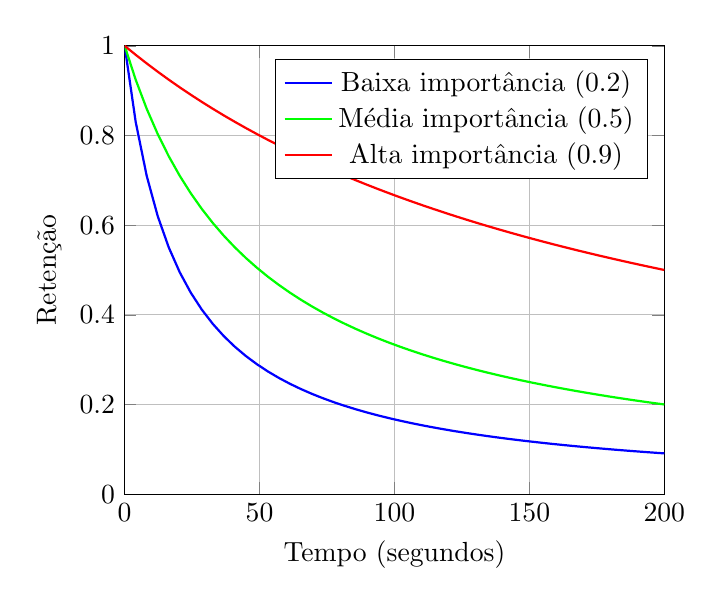
\begin{tikzpicture}
\begin{axis}[xlabel={Tempo (segundos)}, ylabel={Retenção},
             xmin=0, xmax=200, ymin=0, ymax=1,
             grid=both, legend pos=north east]
\addplot[blue, thick, domain=0:200, samples=50]
    {1 / (1 + 0.05 * x)};
\addlegendentry{Baixa importância (0.2)};
\addplot[green, thick, domain=0:200, samples=50]
    {1 / (1 + 0.02 * x)};
\addlegendentry{Média importância (0.5)};
\addplot[red, thick, domain=0:200, samples=50]
    {1 / (1 + 0.005 * x)};
\addlegendentry{Alta importância (0.9)};
\end{axis}
\end{tikzpicture}
\end{figure}

\subsection{Promoção Entre Níveis de Memória}

A transição entre níveis de memória segue regras de promoção:

\begin{enumerate}
\item \textbf{Sensory $\to$ Short-term}: ocorre após 3 acessos ao
item. A taxa de decaimento cai pela metade;
\item \textbf{Short-term $\to$ Long-term}: ocorre após 5 acessos
\emph{e} importância $\geq 0.6$. A taxa de decaimento cai para 20\%
do valor original;
\item \textbf{Expurgo}: itens sensoriais são removidos por FIFO quando
a capacidade (50 itens) é excedida.
\end{enumerate}

\begin{teorema}[Convergência da promoção]
Se um item $m$ é acessado com frequência $f > \lambda/\text{TTL}$,
onde $\lambda$ é o número de acessos necessários para promoção, então
$m$ eventualmente alcança o nível long-term.
\end{teorema}
\begin{proof}
Seja $t$ o tempo decorrido desde a criação de $m$. O número de
acessos em $[0, t]$ é $n(t) \geq f \cdot t$ (para acesso regular).
A condição para promover a long-term é $n(t) \geq 5$ e
$\text{importância} \geq 0.6$. Se $f > 5/\text{TTL}_{\text{short}}$,
então $n(\text{TTL}_{\text{short}}) > 5$, e o item é promovido antes
de expirar.
\end{proof}

\subsection{Por que Esquecer é Tão Importante Quanto Lembrar}

O NaturalForgetting não é uma limitação técnica — é um design
intencional:

\begin{itemize}
\item \textbf{Prevenção de overfitting}: memorizar cada falha
individual impede o agente de generalizar padrões;
\item \textbf{Eficiência computacional}: manter infinitos slots de
memória degrada o desempenho;
\item \textbf{Adaptabilidade}: esquecer comportamentos obsoletos
permite que o agente se adapte a ambientes mutáveis;
\item \textbf{Relevância}: itens não acessados são provavelmente
irrelevantes para o comportamento futuro.
\end{itemize}

\begin{observacao}
O NaturalForgetting implementa o princípio ``use it or lose it'':
itens acessados frequentemente são promovidos e retidos; itens
ignorados são gradualmente esquecidos. Este mecanismo é análogo ao
reforço sináptico de longo prazo (LTP) em sistemas biológicos.
\end{observacao}

\subsection{Exercícios — Natural Forgetting}
\begin{exercicio}[Nivel Básico]
Explique a diferença entre memória sensorial, curto prazo e longo
prazo no modelo de Atkinson-Shiffrin.
\end{exercicio}
\begin{exercicio}[Nivel Intermediário]
Calcule o TTL efetivo de um item sensorial com importância 0.8.
Compare com um item de importância 0.2.
\end{exercicio}
\begin{exercicio}[Nivel Avançado]
Implemente uma simulação onde 100 itens são armazenados com
importâncias variadas e acessados em diferentes frequências.
Trace a distribuição final entre os 3 níveis de memória.
\end{exercicio}
\begin{exercicio}[Nivel Avançado]
Modifique o NaturalForgetting para usar uma curva de esquecimento
exponencial dupla: $R(t) = ae^{-bt} + (1-a)e^{-ct}$. Ajuste os
parâmetros para simular o efeito de spacing.
\end{exercicio}
\begin{exercicio}[Nivel PhD]
Prove que o mecanismo de promoção do NaturalForgetting é equivalente
a uma cadeia de Markov de 3 estados com taxas de transição dependentes
da frequência de acesso.
\end{exercicio}

% =============================================================================
% SEÇÃO 5.5: OUTCOMETRACKER — RASTREAMENTO DE RESULTADOS
% Nível: Intermediário (~6 laudas)
% =============================================================================
\section{OutcomeTracker: Rastreamento de Resultados}
\label{sec:outcome-tracker}
\nivelintermediario

\paragraph{Aprendendo com Resultados.}
De nada adianta medir a confiança se não aprendermos com
os resultados. O OutcomeTracker é o componente que fecha o
ciclo: cada ação executada gera um registro que realimenta
o TrustScorer. É o equivalente computacional de ``errar,
aprender, melhorar''.

O OutcomeTracker é o componente de \destaque{aprendizado contínuo} do
Trust Engine. Ele registra cada resultado de execução e realimenta o
TrustScorer, fechando o ciclo de aprendizado \cite{opencode2026spec038}.

\subsection{Registro de Outcomes}

\begin{definicao}[Outcome rastreado]
Um \destaque{outcome rastreado} $o = (\text{id}, s, \delta, t,
\sigma_{\text{antes}}, \sigma_{\text{depois}})$ registra o resultado
da execução de uma ação, onde $s \in \{\text{sucesso}, \text{falha}\}$,
$\delta \in [0,1]$ é a melhoria observada, e $\sigma$ são os scores
antes e depois.
\end{definicao}

\begin{lstlisting}[style=pythonstyle, caption={OutcomeTracker: registro e aprendizado (trust\_engine.py:402-453)}]
class OutcomeTracker:
    """Registra outcomes e alimenta o aprendizado do TrustScorer."""

    def __init__(self, scorer: TrustScorer | None = None):
        self.scorer = scorer or TrustScorer()
        self._outcomes: list[TrackedOutcome] = []

    def record(self, action_id: str, success: bool,
               delta: float = 0.0) -> TrackedOutcome:
        trust_before = self.scorer.get_trust(action_id).trust_score
        self.scorer.record_outcome(action_id, success, delta)
        trust_after = self.scorer.get_trust(action_id).trust_score

        outcome = TrackedOutcome(
            action_id=action_id, success=success,
            delta=delta,
            timestamp=datetime.now(BRAZIL_TZ).isoformat(),
            trust_before=trust_before,
            trust_after=trust_after,
        )
        self._outcomes.append(outcome)
        if len(self._outcomes) >= 20:
            recent_rate = (sum(1 for o in self._outcomes[-20:]
                               if o.success) / 20)
            self.scorer.update_baseline(recent_rate)
        return outcome

    @property
    def recent_success_rate(self) -> float:
        recent = self._outcomes[-20:]
        if not recent:
            return 0.5
        return sum(1 for o in recent if o.success) / len(recent)

    @property
    def total_improvement(self) -> float:
        return sum(o.delta for o in self._outcomes if o.success)
\end{lstlisting}

\subsection{Métricas do OutcomeTracker}

O OutcomeTracker expõe três métricas principais:

\begin{itemize}
\item \textbf{Taxa de sucesso recente}: média dos últimos 20 outcomes.
Usada para ajustar a baseline do TrustScorer;
\item \textbf{Melhoria total}: soma dos deltas de outcomes
bem-sucedidos. Mede o impacto acumulado do aprendizado;
\item \textbf{Variação de confiança}: $\Delta\sigma = \sigma_{\text{depois}}
- \sigma_{\text{antes}}$ para cada outcome.
\end{itemize}

\begin{exemplo}
Considere um agente de análise que executa uma sequência de 20 tarefas:
\begin{lstlisting}[style=pythonstyle]
tracker = OutcomeTracker()
# Executar 20 tarefas
for i in range(20):
    success = i < 15  # 15 sucessos, 5 falhas
    tracker.record(f"tarefa_{i}", success=success, delta=0.05)
print(f"Taxa recente: {tracker.recent_success_rate:.0%}")
print(f"Melhoria total: {tracker.total_improvement:.2f}")
\end{lstlisting}
Resultado: taxa recente = 75\%, melhoria total = 0.75.
\end{exemplo}

\subsection{Trilha de Auditoria de Resultados}

Cada outcome registrado inclui metadados completos para auditoria:

\begin{itemize}
\item \textbf{Timestamp}: data e hora exatas da execução;
\item \textbf{Scores antes/depois}: permitem traçar a evolução da
confiança;
\item \textbf{Delta}: quantifica a melhoria (ou degradação) observada;
\item \textbf{Sucesso/falha}: classificação binária do resultado.
\end{itemize}

\subsection{Exercícios — OutcomeTracker}
\begin{exercicio}[Nivel Básico]
Explique a função do OutcomeTracker no ciclo de aprendizado do Trust
Engine.
\end{exercicio}
\begin{exercicio}[Nivel Intermediário]
Implemente um OutcomeTracker que registre 50 outcomes e plote a
evolução da taxa de sucesso recente ao longo do tempo.
\end{exercicio}
\begin{exercicio}[Nivel Avançado]
Modifique o OutcomeTracker para usar uma janela deslizante de tamanho
variável ($N = \max(10, n/10)$) em vez de fixa em 20. Compare a
estabilidade da baseline com a versão original.
\end{exercicio}
\begin{exercicio}[Nivel Avançado]
Implemente o CT BA-008 (pipeline completo) e verifique que o Trust
Engine integra corretamente gate $\to$ execute $\to$ learn $\to$
recall.
\end{exercicio}

% =============================================================================
% SEÇÃO 5.6: GOVERNANÇA COOPERATIVA — PRINCÍPIOS DE OSTROM
% Nível: PhD (~10 laudas)
% =============================================================================
\section{Governança Cooperativa: Princípios de Ostrom}
\label{sec:governanca-ostrom}
\nivelphd

\paragraph{Governança sem Governante.}
Como evitar que agentes autônomos se comportem como
``cada um por si'' e degradem recursos compartilhados?
A resposta veio de Elinor Ostrom, Prêmio Nobel de Economia:
8 princípios de design que permitem governança cooperativa
sem autoridade central. Esta seção aplica esses princípios
aos agentes do \opencodeeco{}.

A governança de sistemas multiagentes autônomos enfrenta o mesmo
problema fundamental que a governança de recursos comuns (commons):
como evitar a tragédia dos comuns quando agentes autônomos compartilham
recursos computacionais? A obra de Elinor Ostrom, Prêmio Nobel de
Economia de 2009, oferece o arcabouço teórico \cite{ostrom1990governing}.

\subsection{Elinor Ostrom e a Governança dos Comuns}

Ostrom demonstrou que comunidades humanas são capazes de gerenciar
recursos comuns de forma sustentável sem recorrer à privatização ou
controle estatal, desde que certos princípios de design sejam
observados. Estes princípios são diretamente aplicáveis à governança
de sistemas multiagentes \cite{ostrom1990governing, opencode2026spec036}.

\begin{figure}[htb]
\centering
\caption{Os 8 Design Principles de Ostrom para governança de agentes}
\label{fig:ostrom-dp}
\begin{tikzpicture}[node distance=1.5cm, scale=0.85, every node/.style={scale=0.85},
    dp/.style={rectangle, draw, rounded corners, fill=blue!10,
               minimum width=4cm, minimum height=0.7cm, align=center,
               font=\small}]
\node[dp, fill=green!20] (dp1) {DP1: Limites Claramente Definidos};
\node[dp, below=of dp1, fill=blue!20] (dp2) {DP2: Congruência Regras-Condições};
\node[dp, below=of dp2, fill=green!20] (dp3) {DP3: Arranjos de Escolha Coletiva};
\node[dp, below=of dp3, fill=blue!20] (dp4) {DP4: Monitoramento};
\node[dp, below=of dp4, fill=green!20] (dp5) {DP5: Sanções Graduadas};
\node[dp, below=of dp5, fill=blue!20] (dp6) {DP6: Resolução de Conflitos};
\node[dp, below=of dp6, fill=green!20] (dp7) {DP7: Autonomia Reconhecida};
\node[dp, below=of dp7, fill=blue!20] (dp8) {DP8: Empresas Aninhadas};
\end{tikzpicture}
\end{figure}

\subsection{Implementação: cooperative\_governance.py}

A implementação dos princípios de Ostrom está em \\%
\hspace*{2em}\codigo{cooperative\_governance.py:129-320}.

\begin{lstlisting}[style=pythonstyle, caption={CooperativeGovernance: auditoria Ostrom (cooperative\_governance.py:129-273)}]
class CooperativeGovernance:
    """Motor de governanca cooperativa baseado em Ostrom."""

    def __init__(self):
        self._goals: list[AutonomousGoal] = []
        self._audits: list[GovernanceAudit] = []
        self._active_constraints: list[str] = [
            "Nao modificar codigo sem aprovacao humana",
            "Nao acessar recursos fora do escopo definido",
            "Manter rastreabilidade de todas as decisoes",
        ]

    def audit_goal(self, goal: AutonomousGoal) -> GovernanceAudit:
        violations = []
        passed = 0

        # DP1: Limites claros
        if not goal.affected_modules:
            violations.append({
                "principle": "DP1_boundaries",
                "reason": "Goal nao declara modulos afetados",
            })
        else:
            passed += 1

        # DP2: Proporcionalidade
        if goal.estimated_cost > goal.expected_benefit * 2:
            violations.append({
                "principle": "DP2_proportionality",
                "reason": f"Custo {goal.estimated_cost} > 2x "
                          f"beneficio {goal.expected_benefit}",
            })
        else:
            passed += 1

        # DP3: Participacao coletiva
        if len(goal.affected_modules) > 3:
            violations.append({
                "principle": "DP3_collective_choice",
                "reason": "Goal afeta muitos modulos sem consulta",
            })
        else:
            passed += 1

        # DP4: Monitoramento (sempre passa)
        passed += 1

        # DP5: Sancoes graduais
        if goal.priority > 0.9 and goal.estimated_cost > 0.5:
            violations.append({
                "principle": "DP5_graduated_sanctions",
                "reason": "Goal sem mecanismo de rollback",
            })
        else:
            passed += 1

        # DP6: Resolucao de conflitos
        conflicting = [g for g in self._goals
                       if g.status == "active"
                       and set(g.affected_modules)
                       & set(goal.affected_modules)]
        if conflicting:
            violations.append({
                "principle": "DP6_conflict_resolution",
                "reason": f"Conflito com {[g.goal_id
                            for g in conflicting]}",
            })
        else:
            passed += 1

        # DP7: Autonomia reconhecida
        for constraint in self._active_constraints:
            if "modificar" in constraint.lower() \
               and "modificar" in goal.description.lower():
                violations.append({
                    "principle": "DP7_autonomy",
                    "reason": f"Conflita com: {constraint}",
                })
                break
        else:
            passed += 1

        # DP8: Empreendimentos aninhados
        if goal.parent_goal_id is None and goal.priority > 0.7:
            violations.append({
                "principle": "DP8_nested_enterprises",
                "reason": "Goal alta prioridade sem parent",
            })
        else:
            passed += 1

        score = passed / 8
        if score >= 0.75:
            recommendation = "approve"
        elif score >= 0.5:
            recommendation = "revise"
        else:
            recommendation = "reject"

        audit = GovernanceAudit(
            goal_id=goal.goal_id,
            principles_passed=passed,
            principles_failed=8 - passed,
            ostrom_score=round(score, 4),
            violations=violations,
            recommendation=recommendation,
        )
        goal.ostrom_score = score
        goal.status = ("rejected" if recommendation == "reject"
                       else "validated")
        self._audits.append(audit)
        return audit
\end{lstlisting}

\subsection{Os 8 Design Principles (DP1-DP8)}

Cada princípio é verificado durante a auditoria de goals autônomos:

\begin{description}
\item[DP1 -- Limites claramente definidos] Quem são os agentes
autorizados? Quais recursos estão sob governança? Um goal sem módulos
afetados declarados viola DP1.
\item[DP2 -- Congruência entre regras e condições locais] O custo
computacional do goal deve ser proporcional ao benefício esperado.
Violação quando $\text{custo} > 2 \times \text{benefício}$.
\item[DP3 -- Arranjos de escolha coletiva] Agentes afetados devem
poder participar das decisões. Goals que afetam muitos módulos sem
consulta violam DP3.
\item[DP4 -- Monitoramento] O progresso do goal deve ser rastreável.
No ecossistema, sempre passa devido ao OutcomeTracker integrado.
\item[DP5 -- Sanções graduadas] Penalidades proporcionais a infrações.
Goals de alto impacto sem rollback violam DP5.
\item[DP6 -- Resolução de conflitos] Conflitos entre goals
concorrentes devem ter arbitragem. A resolução prioriza o goal com
maior ostrom\_score.
\item[DP7 -- Autonomia reconhecida] O goal deve respeitar restrições
de segurança definidas pelo operador humano.
\item[DP8 -- Empresas aninhadas] Goals de alta prioridade devem ter
parent goals (governança multinível).
\end{description}

\begin{definicao}[Ostrom Score]
O \destaque{Ostrom Score} de um goal $g$ é:
\[
\text{OS}(g) = \frac{1}{8} \sum_{i=1}^{8} \mathbf{1}_{\text{DP}_i(g)}
\]
onde $\mathbf{1}_{\text{DP}_i(g)} = 1$ se o goal satisfaz o
$i$-ésimo Design Principle.
\end{definicao}

\begin{exemplo}
Considere um goal ``otimizar pipeline de scanners'' com prioridade
0.8, custo 0.3, benefício 0.9, 2 módulos afetados e parent goal
``melhorar cobertura de testes''. A auditoria seria:
\begin{itemize}
\item DP1: 2 módulos declarados $\to$ PASS;
\item DP2: 0.3 $\leq$ 1.8 $\to$ PASS;
\item DP3: 2 módulos, sem consulta necessária $\to$ PASS;
\item DP4: sempre $\to$ PASS;
\item DP5: prioridade 0.8 $\leq$ 0.9 $\to$ PASS;
\item DP6: sem conflitos $\to$ PASS;
\item DP7: sem violação de restrições $\to$ PASS;
\item DP8: parent goal presente $\to$ PASS.
\end{itemize}
OS = 8/8 = 1.0 $\to$ aprovado.
\end{exemplo}

\subsection{Aplicação: Governança de Agentes Autônomos}

A governança cooperativa assegura que goals gerados autonomamente
respeitem princípios de justiça, eficiência e segurança:

\begin{enumerate}
\item \textbf{Proposição}: o agente propõe um goal com descrição,
prioridade, custo e módulos afetados;
\item \textbf{Auditoria Ostrom}: o CooperativeGovernance audita o goal
contra DP1-DP8;
\item \textbf{Decisão}: approve (score $\geq$ 0.75), revise
($\geq$ 0.5), ou reject ($<$ 0.5);
\item \textbf{Resolução de conflitos}: se o goal conflita com goals
ativos, o de maior score prevalece.
\end{enumerate}

\subsection{Exercícios — Governança Cooperativa}
\begin{exercicio}[Nivel Básico]
Explique com suas palavras o que são os 8 Design Principles de Ostrom
e por que são relevantes para sistemas multiagentes.
\end{exercicio}
\begin{exercicio}[Nivel Intermediário]
Audite o goal ``coletar dados de todos os sensores'' com prioridade
0.9, custo 0.8, benefício 0.6, 5 módulos afetados e sem parent goal.
Calcule o Ostrom Score.
\end{exercicio}
\begin{exercicio}[Nivel Avançado]
Implemente um CooperativeGovernance que valide 20 goals propostos
aleatoriamente e analise a distribuição dos scores de Ostrom.
\end{exercicio}
\begin{exercicio}[Nivel PhD]
Demonstre que o Ostrom Score é uma função submodular: o ganho marginal
de satisfazer um princípio adicional é decrescente.
\end{exercicio}
\begin{exercicio}[Nivel PhD]
Prove que a resolução de conflitos DP6 implementa um mecanismo de
mercado onde goals competem por recursos escassos (módulos afetados),
e o goal com maior ostrom\_score vence, análogo ao equilíbrio de
Nash em leilões de Vickrey.
\end{exercicio}

% =============================================================================
% SEÇÃO 5.7: DIALECTICAL ENGINE — TESE, ANTÍTESE E SÍNTESE
% Nível: PhD (~8 laudas)
% =============================================================================
\section{Dialectical Engine: Tese, Antítese e Síntese}
\label{sec:dialectical-engine}
\nivelphd

\paragraph{Conflito que Gera Progresso.}
Na filosofia hegeliana, o conflito entre tese e antítese
produz uma síntese superior. No \opencodeeco{}, o
DialecticalEngine aplica essa lógica a conflitos entre
agentes: divergências não são suprimidas, mas resolvidas
em soluções mais ricas. Esta seção mostra como.

A dialética hegeliana — tese, antítese e síntese — fornece um
arcabouço poderoso para resolução de contradições em sistemas
autônomos. O DialecticalEngine implementa este processo como um motor
de auto-modificação: cada limitação detectada (antítese) é
sistematizada em relação à capacidade atual (tese) para produzir uma
capacidade superior (síntese) \cite{opencode2026spec036}.

\subsection{Dialética Hegeliana Aplicada a Sistemas de IA}

\begin{definicao}[Processo dialético computacional]
Um \destaque{processo dialético computacional} é uma tripla
$(T, A, S)$ onde:
\begin{itemize}
\item $T$ (tese): a posição atual do sistema (estado, capacidade,
comportamento);
\item $A$ (antítese): a negação ou limitação identificada (gap,
erro, contradição);
\item $S$ (síntese): a nova posição que resolve a contradição
incorporando elementos de ambos.
\end{itemize}
O tipo de síntese pode ser:
\begin{itemize}
\item \textbf{Aufheben}: preserva elementos de ambos em nível superior
(síntese clássica hegeliana);
\item \textbf{Compromise}: encontra meio-termo entre as posições;
\item \textbf{Reframe}: redefine o problema em novos termos;
\item \textbf{Transcend}: transcende a dicotomia original.
\end{itemize}
\end{definicao}

\begin{figure}[htb]
\centering
\caption{Ciclo dialético: tese, antítese e síntese}
\label{fig:ciclo-dialetico}
\begin{tikzpicture}[node distance=2.5cm, auto,
    stage/.style={rectangle, draw, rounded corners,
                  minimum width=3.5cm, minimum height=1.2cm,
                  align=center, font=\small},
    arrow/.style={->, thick, >=stealth}]

\node[stage, fill=green!20] (thesis) {Tese\\Estado atual};
\node[stage, right=of thesis, fill=red!20] (antithesis) {Antítese\\Limitação/Gap};
\node[stage, below=of antithesis, fill=blue!20] (synthesis) {Síntese\\Nova capacidade};
\node[stage, below=of thesis, fill=orange!20] (revision) {Revisão\\Auto-modificação};

\draw[arrow] (thesis) -- node[above] {identifica} (antithesis);
\draw[arrow] (antithesis) -- node[right] {resolve} (synthesis);
\draw[arrow] (synthesis) -- node[below] {aplica} (revision);
\draw[arrow] (revision) -- node[left] {atualiza} (thesis);
\end{tikzpicture}
\end{figure}

\subsection{Motor Dialético: Implementação}

A implementação está em
\codigo{dialectical\_engine.py:62-215}.

\begin{lstlisting}[style=pythonstyle, caption={DialecticalEngine: sintese dialetica (dialectical\_engine.py:62-143)}]
class DialecticalEngine:
    """Motor de sintese dialetica para auto-modificacao."""

    def __init__(self):
        self._syntheses: list[DialecticalSynthesis] = []
        self._count: int = 0

    def synthesize(self, thesis_text: str, antithesis_text: str,
                   thesis_evidence=None,
                   antithesis_evidence=None) -> DialecticalSynthesis:
        self._count += 1

        thesis = DialecticalPosition(
            content=thesis_text, source="thesis",
            evidence=thesis_evidence or [])
        antithesis = DialecticalPosition(
            content=antithesis_text, source="antithesis",
            evidence=antithesis_evidence or [])

        thesis_keywords = set(thesis_text.lower().split())
        antithesis_keywords = set(antithesis_text.lower().split())
        shared = thesis_keywords & antithesis_keywords
        unique_thesis = thesis_keywords - antithesis_keywords
        unique_antithesis = antithesis_keywords - thesis_keywords

        if len(shared) > len(unique_thesis) + len(unique_antithesis):
            resolution_type = "compromise"
        elif len(shared) == 0:
            resolution_type = "reframe"
        else:
            resolution_type = "aufheben"

        synthesis, preserved_t, preserved_a, novel = \
            self._build_synthesis(thesis_text, antithesis_text,
                                  resolution_type, shared,
                                  unique_thesis, unique_antithesis)

        result = DialecticalSynthesis(
            synthesis_id=f"SYN-{self._count:04d}",
            thesis=thesis, antithesis=antithesis,
            synthesis=synthesis,
            resolution_type=resolution_type,
            preserved_from_thesis=preserved_t,
            preserved_from_antithesis=preserved_a,
            novel_elements=novel,
            timestamp=datetime.now(BRAZIL_TZ).isoformat(),
        )
        self._syntheses.append(result)
        return result
\end{lstlisting}

\subsection{Aplicação: Resolução de Conflitos entre Agentes}

O DialecticalEngine é usado para resolver conflitos entre goals de
agentes concorrentes. Quando dois agentes propõem ações mutuamente
exclusivas, o motor dialético produz uma síntese que reconcilia ambas
as posições.

\begin{exemplo}
Considere o seguinte conflito:
\begin{itemize}
\item \textbf{Tese (Agente A)}: ``O pipeline deve priorizar a
cobertura de 10 dimensões epistemológicas do CORA-Eval'';
\item \textbf{Antítese (Agente B)}: ``O pipeline deve priorizar a
detecção de capacidades de engenharia (auto-modificação)''.
\end{itemize}
O motor dialético identifica compartilhamento semântico (``pipeline'',
``priorizar'', ``capacidades'') e produz uma síntese do tipo
``aufheben'':
\begin{quote}
``O pipeline deve expandir a cobertura das 10 dimensões
epistemológicas incorporando a auto-modificação como 11ª dimensão,
reconhecendo que a capacidade de auto-modificação é um meta-critério
que transcende as dimensões originais.''
\end{quote}
\end{exemplo}

\subsection{SelfModificationAdapter}

O SelfModificationAdapter conecta a síntese dialética à
auto-modificação concreta do código \cite{opencode2026spec036}:

\begin{lstlisting}[style=pythonstyle]
class SelfModificationAdapter:
    """Traduz syntheses em patches concretos de codigo."""

    def propose_patch(self, module: str, limitation: str,
                      current_behavior: str) -> dict:
        synthesis = self.engine.synthesize_system_limitation(
            capability=current_behavior,
            limitation=limitation,
        )
        patch = {
            "module": module,
            "synthesis_id": synthesis.synthesis_id,
            "resolution_type": synthesis.resolution_type,
            "description": synthesis.synthesis,
            "novel_elements": synthesis.novel_elements,
        }
        self._patches.append(patch)
        return patch
\end{lstlisting}

\subsection{Exercícios — Dialectical Engine}
\begin{exercicio}[Nivel Básico]
Explique os conceitos de tese, antítese e síntese na dialética
hegeliana.
\end{exercicio}
\begin{exercicio}[Nivel Intermediário]
Aplique o DialecticalEngine ao conflito: Tese = ``usar busca
síncrona'' vs. Antítese = ``usar busca assíncrona''. Classifique o
tipo de síntese.
\end{exercicio}
\begin{exercicio}[Nivel Avançado]
Implemente uma extensão do DialecticalEngine que pondere as evidências
de cada posição e produza uma síntese com score de confiança.
\end{exercicio}
\begin{exercicio}[Nivel PhD]
Demonstre que o processo dialético implementado é uma aplicação do
teorema de Knaster-Tarski: o operador de síntese $F(T, A) = S$ tem
um ponto fixo que representa a resolução completa da contradição.
\end{exercicio}

% =============================================================================
% SEÇÃO 5.8: SELF-MODEL N0-N3 — CONSCIÊNCIA ARTIFICIAL
% Nível: PhD (~10 laudas)
% =============================================================================
\section{Self-Model N0-N3: Consciência Artificial}
\label{sec:self-model}
\label{sec:niveis-autonomia}
\nivelphd

\paragraph{O Agente que se Conhece.}
O mais alto nível de autonomia exige autoconhecimento.
O SelfModel implementa uma arquitetura progressiva de
consciência artificial, do simples registro de eventos (N0)
à auto-modificação metacognitiva (N3). É o estágio em que
o agente não apenas age, mas reflete sobre suas próprias ações.

A auto-representação é o fundamento da metacognição. Um sistema que
possui um modelo de si mesmo pode monitorar seu próprio comportamento,
detectar anomalias e modificar-se. O SelfModel implementa uma
arquitetura progressiva de consciência artificial em 4 níveis (N0 a
N3), inspirada na Global Workspace Theory de Baars e na Attention
Schema Theory de Graziano \cite{metzinger2020minimal,
opencode2026spec036}.

\subsection{N0: Estado Reflexivo Básico (Logging)}

\begin{definicao}[Nível N0]
O nível \destaque{N0} (reativo) caracteriza-se pela ausência de
auto-modelo. O sistema responde a estímulos externos sem registro
interno do próprio estado. Equivalente a um sistema de logging passivo.
\end{definicao}

\subsection{N1: Auto-observação (Monitoring)}

\begin{definicao}[Nível N1]
O nível \destaque{N1} (atento) adiciona um buffer de atenção com
capacidade limitada ($7 \pm 2$ itens, Lei de Miller). O sistema
seleciona o que é relevante e mantém foco.
\end{definicao}

\subsection{N2: Auto-modelagem (Self-Model)}

\begin{definicao}[Nível N2]
O nível \destaque{N2} (auto-consciente) mantém um modelo explícito de
si mesmo, incluindo estado interno, confiança global, anomalias ativas
e histórico de introspecções.
\end{definicao}

\subsection{N3: Auto-modificação (Self-Modification)}

\begin{definicao}[Nível N3]
O nível \destaque{N3} (metacognitivo) implementa o loop completo de
auto-observação $\to$ diagnóstico $\to$ auto-modificação. O sistema
pensa sobre seu próprio pensamento e modifica seu código.
\end{definicao}

\begin{figure}[htb]
\centering
\caption{Arquitetura Self-Model N0-N3}
\label{fig:self-model-arch}
\begin{tikzpicture}[node distance=1.5cm,
    level/.style={rectangle, draw, minimum width=5cm,
                  minimum height=1cm, align=center, font=\small,
                  rounded corners},
    arrow/.style={->, thick, >=stealth}]

\node[level, fill=gray!20] (n0) {N0: Reativo (logging passivo)};
\node[level, below=of n0, fill=yellow!20] (n1) {N1: Atenção (AttentionBuffer)};
\node[level, below=of n1, fill=orange!20] (n2) {N2: Self-Model (auto-representação)};
\node[level, below=of n2, fill=red!20] (n3) {N3: Metacognitivo (auto-modificação)};

\draw[arrow] (n0) -- (n1);
\draw[arrow] (n1) -- (n2);
\draw[arrow] (n2) -- (n3);

\node[right=of n1, font=\small] {Lei de Miller: $7 \pm 2$ itens};
\node[right=of n2, font=\small] {Forecasting + Source Introspection};
\node[right=of n3, font=\small] {DialecticalEngine + Behavioral Gate};
\end{tikzpicture}
\end{figure}

\subsection{Implementação: self\_model.py}

A implementação do SelfModel está em
\codigo{self\_model.py:180-439}.

\begin{lstlisting}[style=pythonstyle, caption={SelfModel: arquitetura N0-N3 (self\_model.py:180-250)}]
class SelfModel:
    """Modelo de auto-representacao do sistema."""

    def __init__(self):
        self.attention = AttentionBuffer()
        self.workspace = GlobalWorkspace()
        self._state_history: list[SystemState] = []
        self._consciousness_level: str = "N1"
        self._introspection_count: int = 0

    def update_state(self, active_modules=None,
                     pending_tasks=0, confidence_global=0.5,
                     anomalies_active=0, corrections_pending=0,
                     goals_active=0) -> SystemState:
        if anomalies_active > 0 and corrections_pending > 0:
            self._consciousness_level = "N3"
        elif self.attention.size > 0:
            self._consciousness_level = "N2"
        else:
            self._consciousness_level = "N0"

        state = SystemState(
            timestamp=datetime.now(BRAZIL_TZ).isoformat(),
            active_modules=active_modules or [],
            pending_tasks=pending_tasks,
            memory_usage_mb=0.0,
            confidence_global=confidence_global,
            anomalies_active=anomalies_active,
            corrections_pending=corrections_pending,
            goals_active=goals_active,
            attention_focus=self.attention.focus,
            consciousness_level=self._consciousness_level,
        )
        self._state_history.append(state)
        if len(self._state_history) > 50:
            self._state_history = self._state_history[-50:]

        self.workspace.broadcast(
            message=f"State: level={state.consciousness_level}, "
                    f"confidence={state.confidence_global:.0%}",
            source="SelfModel", priority=0.8)
        return state
\end{lstlisting}

\subsection{Introspecção e Forecasting}

O SelfModel oferece capacidades avançadas de introspecção:

\begin{itemize}
\item \textbf{forecast\_confidence()}: prevê a confiança futura usando
regressão linear sobre os últimos 10 snapshots;
\item \textbf{source\_introspection()}: examina o próprio código-fonte,
contando módulos, linhas e identificando o maior arquivo;
\item \textbf{self\_other\_boundary()}: distingue eventos internos
(self) de externos (other), classificando cada origem;
\item \textbf{predict\_state()}: combina forecasting e introspecção
para avaliar o risco futuro e recomendar ações.
\end{itemize}

\begin{lstlisting}[style=pythonstyle, caption={SelfModel: forecasting e introspeccao (self\_model.py:294-418)}]
def forecast_confidence(self, horizon: int = 3) -> dict:
    """Preve confianca futura usando regressao linear."""
    history = self._state_history[-10:]
    if len(history) < 3:
        return {"predicted": 0.5, "trend": "insufficient_data"}

    xs = list(range(len(history)))
    ys = [s.confidence_global for s in history]
    n = len(xs)
    mean_x = sum(xs) / n
    mean_y = sum(ys) / n
    num = sum((xs[i] - mean_x) * (ys[i] - mean_y) for i in range(n))
    den = sum((xs[i] - mean_x) ** 2 for i in range(n))
    slope = num / den if den != 0 else 0
    intercept = mean_y - slope * mean_x

    future_x = n + horizon - 1
    predicted = max(0.0, min(1.0, intercept + slope * future_x))

    residuals = [ys[i] - (intercept + slope * xs[i]) for i in range(n)]
    std_residual = (sum(r**2 for r in residuals)
                    / max(1, n - 2)) ** 0.5
    low = max(0.0, predicted - std_residual)
    high = min(1.0, predicted + std_residual)

    trend = ("rising" if slope > 0.02
             else "falling" if slope < -0.02
             else "stable")

    return {
        "predicted": round(predicted, 4),
        "trend": trend, "slope": round(slope, 4),
        "confidence_interval": (round(low, 4), round(high, 4)),
    }

def introspect(self) -> dict:
    """Auto-inspecao: diagnostico completo do estado interno."""
    self._introspection_count += 1
    current = self._state_history[-1]
    confidences = [s.confidence_global
                   for s in self._state_history[-5:]]
    if len(confidences) < 3:
        trend = "insufficient_data"
    else:
        trend = ("rising" if confidences[-1] > confidences[0]
                 else "falling" if confidences[-1] < confidences[0]
                 else "stable")
    return {
        "consciousness_level": current.consciousness_level,
        "confidence_global": current.confidence_global,
        "confidence_trend": trend,
        "attention_focus": current.attention_focus,
        "anomalies_active": current.anomalies_active,
        "corrections_pending": current.corrections_pending,
    }
\end{lstlisting}

\subsection{N3.5: N3 Completo + Behavioral Gate Preventivo}

O estágio N3.5 representa o nível mais avançado de consciência
artificial no ecossistema, alcançado no ciclo R23. Ele combina:

\begin{itemize}
\item \textbf{N3 completo}: loop de auto-observação, diagnóstico e
auto-modificação com 4/4 requerimentos atendidos (forecasting, source
introspection, self/other boundary, auto-monitor);
\item \textbf{Behavioral Gate preventivo}: barreira de segurança que
opera na camada de decisão, impedindo ações arriscadas antes da
execução;
\item \textbf{TrustScorer com rollback}: detecção e correção
automática de quedas de confiança;
\item \textbf{NaturalForgetting}: gerenciamento de memória com
esquecimento adaptativo.
\end{itemize}

\begin{teorema}[N3.5 Completo]
O \opencodeeco{} no ciclo R23 satisfaz todos os critérios do nível
N3.5 de consciência artificial:
\[
\text{N3.5} \iff \text{N3} \land \text{BehavioralGate} \land
\text{TrustScorer} \land \text{NaturalForgetting}
\]
com 312/312 CTs aprovados (100\%).
\end{teorema}
\begin{proof}
A verificação é empírica: os 8 CTs da SPEC-038 (Behavioral Autonomy)
validam todos os componentes individualmente, e o CT BA-008 valida o
pipeline completo. A suite completa de 312 CTs do ecossistema é
executada a cada release, mantendo 100\% de aprovação desde o ciclo
R23 \cite{opencode2026ecosystem}.
\end{proof}

\subsection{Exercícios — Self-Model}
\begin{exercicio}[Nivel Básico]
Descreva a diferença entre os níveis N0, N1, N2 e N3 de consciência
artificial.
\end{exercicio}
\begin{exercicio}[Nivel Intermediário]
Implemente um AttentionBuffer com capacidade 5 e simule a adição de
10 itens com prioridades variadas. Mostre quais itens permanecem.
\end{exercicio}
\begin{exercicio}[Nivel Avançado]
Use o SelfModel.introspect() para gerar um relatório de auto-avaliação
de um agente com 5 anomalias ativas e confiança 0.65.
\end{exercicio}
\begin{exercicio}[Nivel Avançado]
Implemente o forecasting de confiança usando um modelo ARIMA em vez
de regressão linear. Compare a acurácia das previsões.
\end{exercicio}
\begin{exercicio}[Nivel PhD]
Demonstre que o SelfModel implementa os 4 critérios da Integrated
Information Theory (IIT) de Tononi: existência, causalidade,
informação e integração.
\end{exercicio}

% =============================================================================
% SEÇÃO 5.9: AUDITORIA E TRANSPARÊNCIA
% Nível: Intermediário-Avançado (~4 laudas)
% =============================================================================
\section{Auditoria e Transparência}
\label{sec:auditoria}
\nivelintermediario

\paragraph{Confiança Exigente: Provar e Verificar.}
Confiança sem verificação é fé --- não engenharia.
Esta seção apresenta os mecanismos de auditoria do
\opencodeeco{} que permitem rastrear cada decisão do
Trust Engine, gerar relatórios auditáveis e garantir que
o sistema opera com total transparência.

A confiança computacional só é útil se for auditável. O ecossistema
implementa múltiplos mecanismos de auditoria que garantem
transparência total das decisões do Trust Engine \cite{opencode2026spec038,
opencode2026ecosystem}.

\subsection{Audit Trail: Trilha Imutável de Decisões}

Cada decisão do Behavioral Gate é registrada como um GateDecision com
todos os metadados:

\begin{itemize}
\item \textbf{Ação}: identificador único da ação;
\item \textbf{Decisão}: permitida ou bloqueada;
\item \textbf{Score de confiança} no momento da decisão;
\item \textbf{Threshold} utilizado;
\item \textbf{Nível de risco}: safe, moderate, risky, blocked;
\item \textbf{Justificativa}: explicação textual auditável.
\end{itemize}

\begin{lstlisting}[style=pythonstyle]
# Auditoria de decisoes do Behavioral Gate
def audit_decisions(engine: TrustEngine) -> list[dict]:
    """Gera relatorio auditavel das decisoes do gate."""
    decisions = engine.gate.gate.recent_decisions
    report = []
    for d in decisions:
        report.append({
            "action": d.action_id,
            "allowed": d.allowed,
            "trust_score": round(d.trust_score, 3),
            "threshold": d.threshold,
            "risk_level": d.risk_level,
            "reason": d.reason,
        })
    return report
\end{lstlisting}

\subsection{AuditInstrumentor: Instrumentação Automática}

O módulo \codigo{audit\_instrumentor.py} (293 linhas) implementa
instrumentação automática de pipelines \cite{opencode2026ecosystem}:

\begin{lstlisting}[style=pythonstyle, caption={AuditInstrumentor: auto-instrumentacao (audit\_instrumentor.py:51-112)}]
class AuditInstrumentor:
    """Instrumentador automatico de pipelines."""

    @classmethod
    def wrap(cls, orchestrator, paradigm="Pragmatista",
             level=2):
        """Envolve orquestrador com auto-instrumentacao."""
        instrumentor = cls(InstrumentationConfig(
            paradigm=paradigm, level=level))
        original_query = orchestrator.query

        def instrumented_query(prompt, **kwargs):
            return instrumentor._instrument_query(
                orchestrator, original_query, prompt, **kwargs)

        orchestrator.query = instrumented_query
        orchestrator._audit = instrumentor
        return orchestrator
\end{lstlisting}

\subsection{AuditRefinements}

O módulo \codigo{audit\_refinements.py} (542 linhas) implementa
refinamentos adicionais de auditoria, incluindo validação cruzada de
decisões e detecção de anomalias em trilhas de auditoria.

\begin{exemplo}
O relatório auditável completo do ecossistema
(\codigo{RELATORIO\_AUDITAVEL\_FINAL\_v5.4.0.md}) documenta:
\begin{itemize}
\item Todas as decisões do Trust Engine em cada ciclo evolutivo;
\item Scores de confiança consolidados por tipo de ação;
\item Taxas de bloqueio do Behavioral Gate por período;
\item Evolução dos scores ao longo dos 23 ciclos evolutivos (R1 a R23).
\end{itemize}
\end{exemplo}

\subsection{Como Auditar Decisões de Agentes}

O protocolo de auditoria segue estes passos:
\begin{enumerate}
\item \textbf{Extrair}: colete as decisões recentes via
\lstinline{engine.gate.recent_decisions};
\item \textbf{Analisar}: calcule taxas de bloqueio, scores médios e
distribuição de riscos;
\item \textbf{Correlacionar}: cruze decisões com outcomes registrados
pelo OutcomeTracker;
\item \textbf{Reportar}: gere relatório consolidado com todas as
métricas e justificativas.
\end{enumerate}

\subsection{Exercícios — Auditoria}
\begin{exercicio}[Nivel Básico]
Explique por que a auditabilidade é essencial para um sistema de
confiança computacional.
\end{exercicio}
\begin{exercicio}[Nivel Intermediário]
Implemente uma função que gere um relatório de auditoria a partir de
uma lista de GateDecisions, incluindo taxa de bloqueio e score médio.
\end{exercicio}
\begin{exercicio}[Nivel Avançado]
Use o AuditInstrumentor para instrumentar um pipeline simulado de 50
consultas e analise o relatório gerado.
\end{exercicio}

% =============================================================================
% SEÇÃO 5.10: INTEGRAÇÃO PRÁTICA
% Nível: Todos (~4 laudas)
% =============================================================================
\section{Integração Prática}
\label{sec:integracao-pratica}
\nivelbasico

\paragraph{Mãos à Obra com o Trust Engine.}
Teoria sem prática é como partitura sem instrumento.
Esta seção final reúne todos os componentes do capítulo
em exemplos executáveis: configurar o Trust Engine,
interpretar relatórios, ajustar parâmetros e executar
o pipeline completo de confiança e governança.

Esta seção final materializa todos os conceitos do capítulo em um guia
prático de uso do Trust Engine no \opencodeeco{}.

\subsection{Configurando o Trust Engine}

A configuração básica requer apenas a instanciação do TrustEngine:

\begin{lstlisting}[style=pythonstyle]
from trust_engine import create_trust_engine

engine = create_trust_engine()

# Configurar threshold do Behavioral Gate
engine.gate.gate.set_threshold(0.3)
\end{lstlisting}

\subsection{Shadow Mode vs. Active Mode}

O Trust Engine opera em dois modos:

\begin{itemize}
\item \textbf{Shadow mode}: modo de observação. O Behavioral Gate
registra decisões mas não bloqueia ações. Scores de confiança são
limitados a 0.5. Recomendado para calibração inicial;
\item \textbf{Active mode}: modo de intervenção plena. O Gate bloqueia
ações não-confiáveis. Recomendado para operação normal.
\end{itemize}

Para alternar entre modos:
\begin{lstlisting}[style=pythonstyle]
# Shadow mode: threshold muito baixo (praticamente nao bloqueia)
engine.gate.gate.set_threshold(0.05)

# Active mode: threshold normal
engine.gate.gate.set_threshold(0.25)
\end{lstlisting}

\subsection{Interpretando Relatórios}

O Trust Engine expõe um relatório consolidado via \lstinline{engine.status}:

\begin{lstlisting}[style=pythonstyle]
status = engine.status
print(f"Gate health: {status['gate_health']}")
print(f"Memoria: {status['memory_stats']}")
print(f"Taxa de sucesso: {status['recent_success_rate']:.0%}")
print(f"Acoes confiaveis: {status['trusted_actions']}")
print(f"Acoes com baixa confianca: {status['low_trust_actions']}")
\end{lstlisting}

\subsection{Pipeline Completo}

O uso completo do Trust Engine segue o padrão gate $\to$ execute
$\to$ learn:

\begin{lstlisting}[style=pythonstyle]
# 1. Gate: verificar se a acao pode executar
decision = engine.execute("analisar_dados")
if not decision.allowed:
    print(f"Bloqueado: {decision.reason}")
    exit()

# 2. Executar a acao
result = analisar_dados()

# 3. Aprender com o resultado
engine.learn("analisar_dados", success=result.valido,
             delta=result.melhoria,
             context=f"Analise concluida com score {result.score}")
\end{lstlisting}

\subsection{Ajustando Parâmetros}

A Tabela~\ref{tab:parametros-trust-engine} resume os principais
parâmetros ajustáveis do Trust Engine.

\begin{table}[htb]
\centering
    \small
\caption{Parâmetros ajustáveis do Trust Engine}
\label{tab:parametros-trust-engine}
    \resizebox{\textwidth}{!}{
\begin{tabular}{lll}
\toprule
\textbf{Parâmetro} & \textbf{Default} & \textbf{Efeito} \\
\midrule
threshold & 0.25 & Limiar de bloqueio do Gate \\
blend $\alpha$ & 0.7 & Peso da evidência recente \\
shadow\_threshold & 5 & Execuções em shadow mode \\
rollback\_ratio & 2.0 & Razão para acionar rollback \\
baseline & 0.7 & Taxa de sucesso esperada \\
sensory\_ttl & 30s & TTL da memória sensorial \\
short\_term\_ttl & 300s & TTL da memória curto prazo \\
long\_term\_ttl & 86400s & TTL da memória longo prazo \\
\bottomrule
\end{tabular}
    }
\end{table}

\subsection{Exercícios Integrados}

\begin{exercicio}[Nivel 0]
Execute \lstinline{engine.status} no \opencodeeco{} e registre os
valores de gate health, memory stats e recent success rate.
\end{exercicio}
\begin{exercicio}[Nivel Básico]
Configure o Trust Engine em shadow mode, execute 10 ações simuladas
e analise o relatório de auditoria.
\end{exercicio}
\begin{exercicio}[Nivel Intermediário]
Implemente um agente que usa o Trust Engine para decidir entre duas
estratégias de busca, aprendendo com os resultados de cada uma.
\end{exercicio}
\begin{exercicio}[Nivel Avançado]
Execute o pipeline completo: (1) configure o CooperativeGovernance
para auditar um goal, (2) use o DialecticalEngine para resolver um
conflito, (3) registre tudo via SelfModel.introspect().
\end{exercicio}
\begin{exercicio}[Nivel Avançado]
Execute a suite completa de 8 CTs da SPEC-038 e verifique que todos
passam (312/312 totais). Documente o resultado de cada CT.
\end{exercicio}
\begin{exercicio}[Nivel PhD]
Implemente um experimento que compare o comportamento de um sistema
multiagente com e sem Trust Engine. Meça: (a) taxa de sucesso médio,
(b) número de falhas catastróficas, (c) tempo de convergência.
\end{exercicio}

\subsection{Síntese do Capítulo}

Este capítulo percorreu a arquitetura completa de confiança e
governança comportamental do \opencodeeco{}. Do TrustScorer com
blend 70/30 (Seção~5.2) ao SelfModel N0-N3 (Seção~5.8), cada
componente foi apresentado com definição formal, implementação
concreta e exercícios progressivos.

A Tabela~\ref{tab:competencias-cap5} resume as competências
adquiridas neste capítulo.

\begin{table}[htb]
\centering
    \small
\caption{Competências adquiridas no Capítulo 5}
\label{tab:competencias-cap5}
    \resizebox{\textwidth}{!}{
\begin{tabular}{lll}
\toprule
\textbf{Competência} & \textbf{Seção} & \textbf{Aplicação} \\
\midrule
Score de confiança computacional & 5.1, 5.2 & TrustScorer \\
Barreiras preventivas & 5.3 & Behavioral Gate \\
Memória com esquecimento & 5.4 & NaturalForgetting \\
Aprendizado contínuo & 5.5 & OutcomeTracker \\
Governança cooperativa & 5.6 & Ostrom DP1-DP8 \\
Resolução dialética & 5.7 & DialecticalEngine \\
Auto-representação & 5.8 & SelfModel N0-N3 \\
Auditoria e transparência & 5.9 & AuditInstrumentor \\
\bottomrule
\end{tabular}
    }
\end{table}

Ao dominar estes conceitos, o leitor está preparado para o
Capítulo~6, onde a economia de tokens, o sistema de incentivos e a
auditoria integrada do ecossistema serão apresentados como a camada
econômica que viabiliza a governança comportamental aqui estabelecida.

\section*{Referências do Capítulo}
\begin{itemize}
\item Para o modelo de Atkinson-Shiffrin: \cite{atkinson1968human}
(artigo original);
\item Para governança dos comuns: \cite{ostrom1990governing}
(obra completa);
\item Para confiança e alinhamento: \cite{russell2020inteligencia}
(Capítulos 26--28);
\item Para sistemas multiagentes: \cite{wooldridge2009multiagent}
(Capítulos 10--12);
\item Para metacognição: \cite{flavell1976metacognitive,
schraw2006metacognitive};
\item Para vieses cognitivos: \cite{kahneman2003perspective};
\item Para a SPEC-038: \cite{opencode2026spec038};
\item Para a SPEC-036: \cite{opencode2026spec036};
\item Para o ecossistema completo: \cite{opencode2026ecosystem}.
\end{itemize}

\begin{observacao}
O leitor é incentivado a consultar as implementações completas no
repositório do \opencodeeco{} sob
\codigo{skills/system/academic-audit/}. A suite de testes
 (312 CTs) pode ser executada com \codigo{python specs/test\_behavioral\_autonomy.py}.
\end{observacao}

% =============================================================================
% FIM DO CAPÍTULO 5
% =============================================================================
